\section{Nuclear fission}
\label{sec:fission}
Nuclear fission is the process by which a nucleus splits into two -- sometimes three -- nuclei, whether spontaneously or when induced by a reaction.
The physics that governs nuclear fission is that of a many-body, large-amplitude collective mode that gradually elongates the nuclear shape until the so-called \textit{fission barrier} is surmounted and the energetically favoured path leads the nucleus to fragment. In figure \ref{fig:fission_barrier}, a graphical representation of the fission path and corresponding barrier is shown.

\begin{figure}[h]
    \centering
    \includegraphics[width=0.8\textwidth]{Images/mocca_barrier.png}
    \caption{Fission path of $^{226}$Ra, blue lines indicate axial octupole configurations, black lines indicate axial quadrupole and parity conserving configurations, red lines indicate triaxial, parity conserving configurations.}
    \label{fig:fission_barrier}
\end{figure}

Although the basic idea of a nucleus dividing into two pieces may appear simple, the underlying dynamics is remarkably rich and involves several stages. Historically, the first theoretical interpretation of fission was given by Bohr and Wheeler in 1939 \cite{BohrWheeler1939_PR56_426}, who formulated the liquid-drop model description and introduced the concept of the fission barrier, determined by the competition between Coulomb repulsion and surface tension. Their framework already suggested that nuclei may experience intermediate configurations, multiple saddle points, and shape isomerism along the fission path.

Subsequent developments incorporated more detailed descriptions of the collective degrees of freedom and the role of shell effects, leading to the recognition that the fission landscape is often characterised by multiple barriers, intermediate minima, and highly deformed transition states \cite{Strutinsky1967_NPA95_420,Brack1972_RMP44_320}. Modern microscopic approaches, based on energy-density functionals, have further clarified that fission dynamics involves a sequence of slow, dissipative shape evolutions, interspersed with possible gamma-decay pathways, and culminating in the formation of two (or more) pre-fragments connected by a narrowing neck. As the system evolves beyond the outer saddle, exotic spatial configurations appear, and the fragments themselves may exhibit deformation or even reflection asymmetry before scission. A visual representation of the overall fission process is shown in figure \ref{fig:fission}.


\begin{figure}[h]
    \centering
    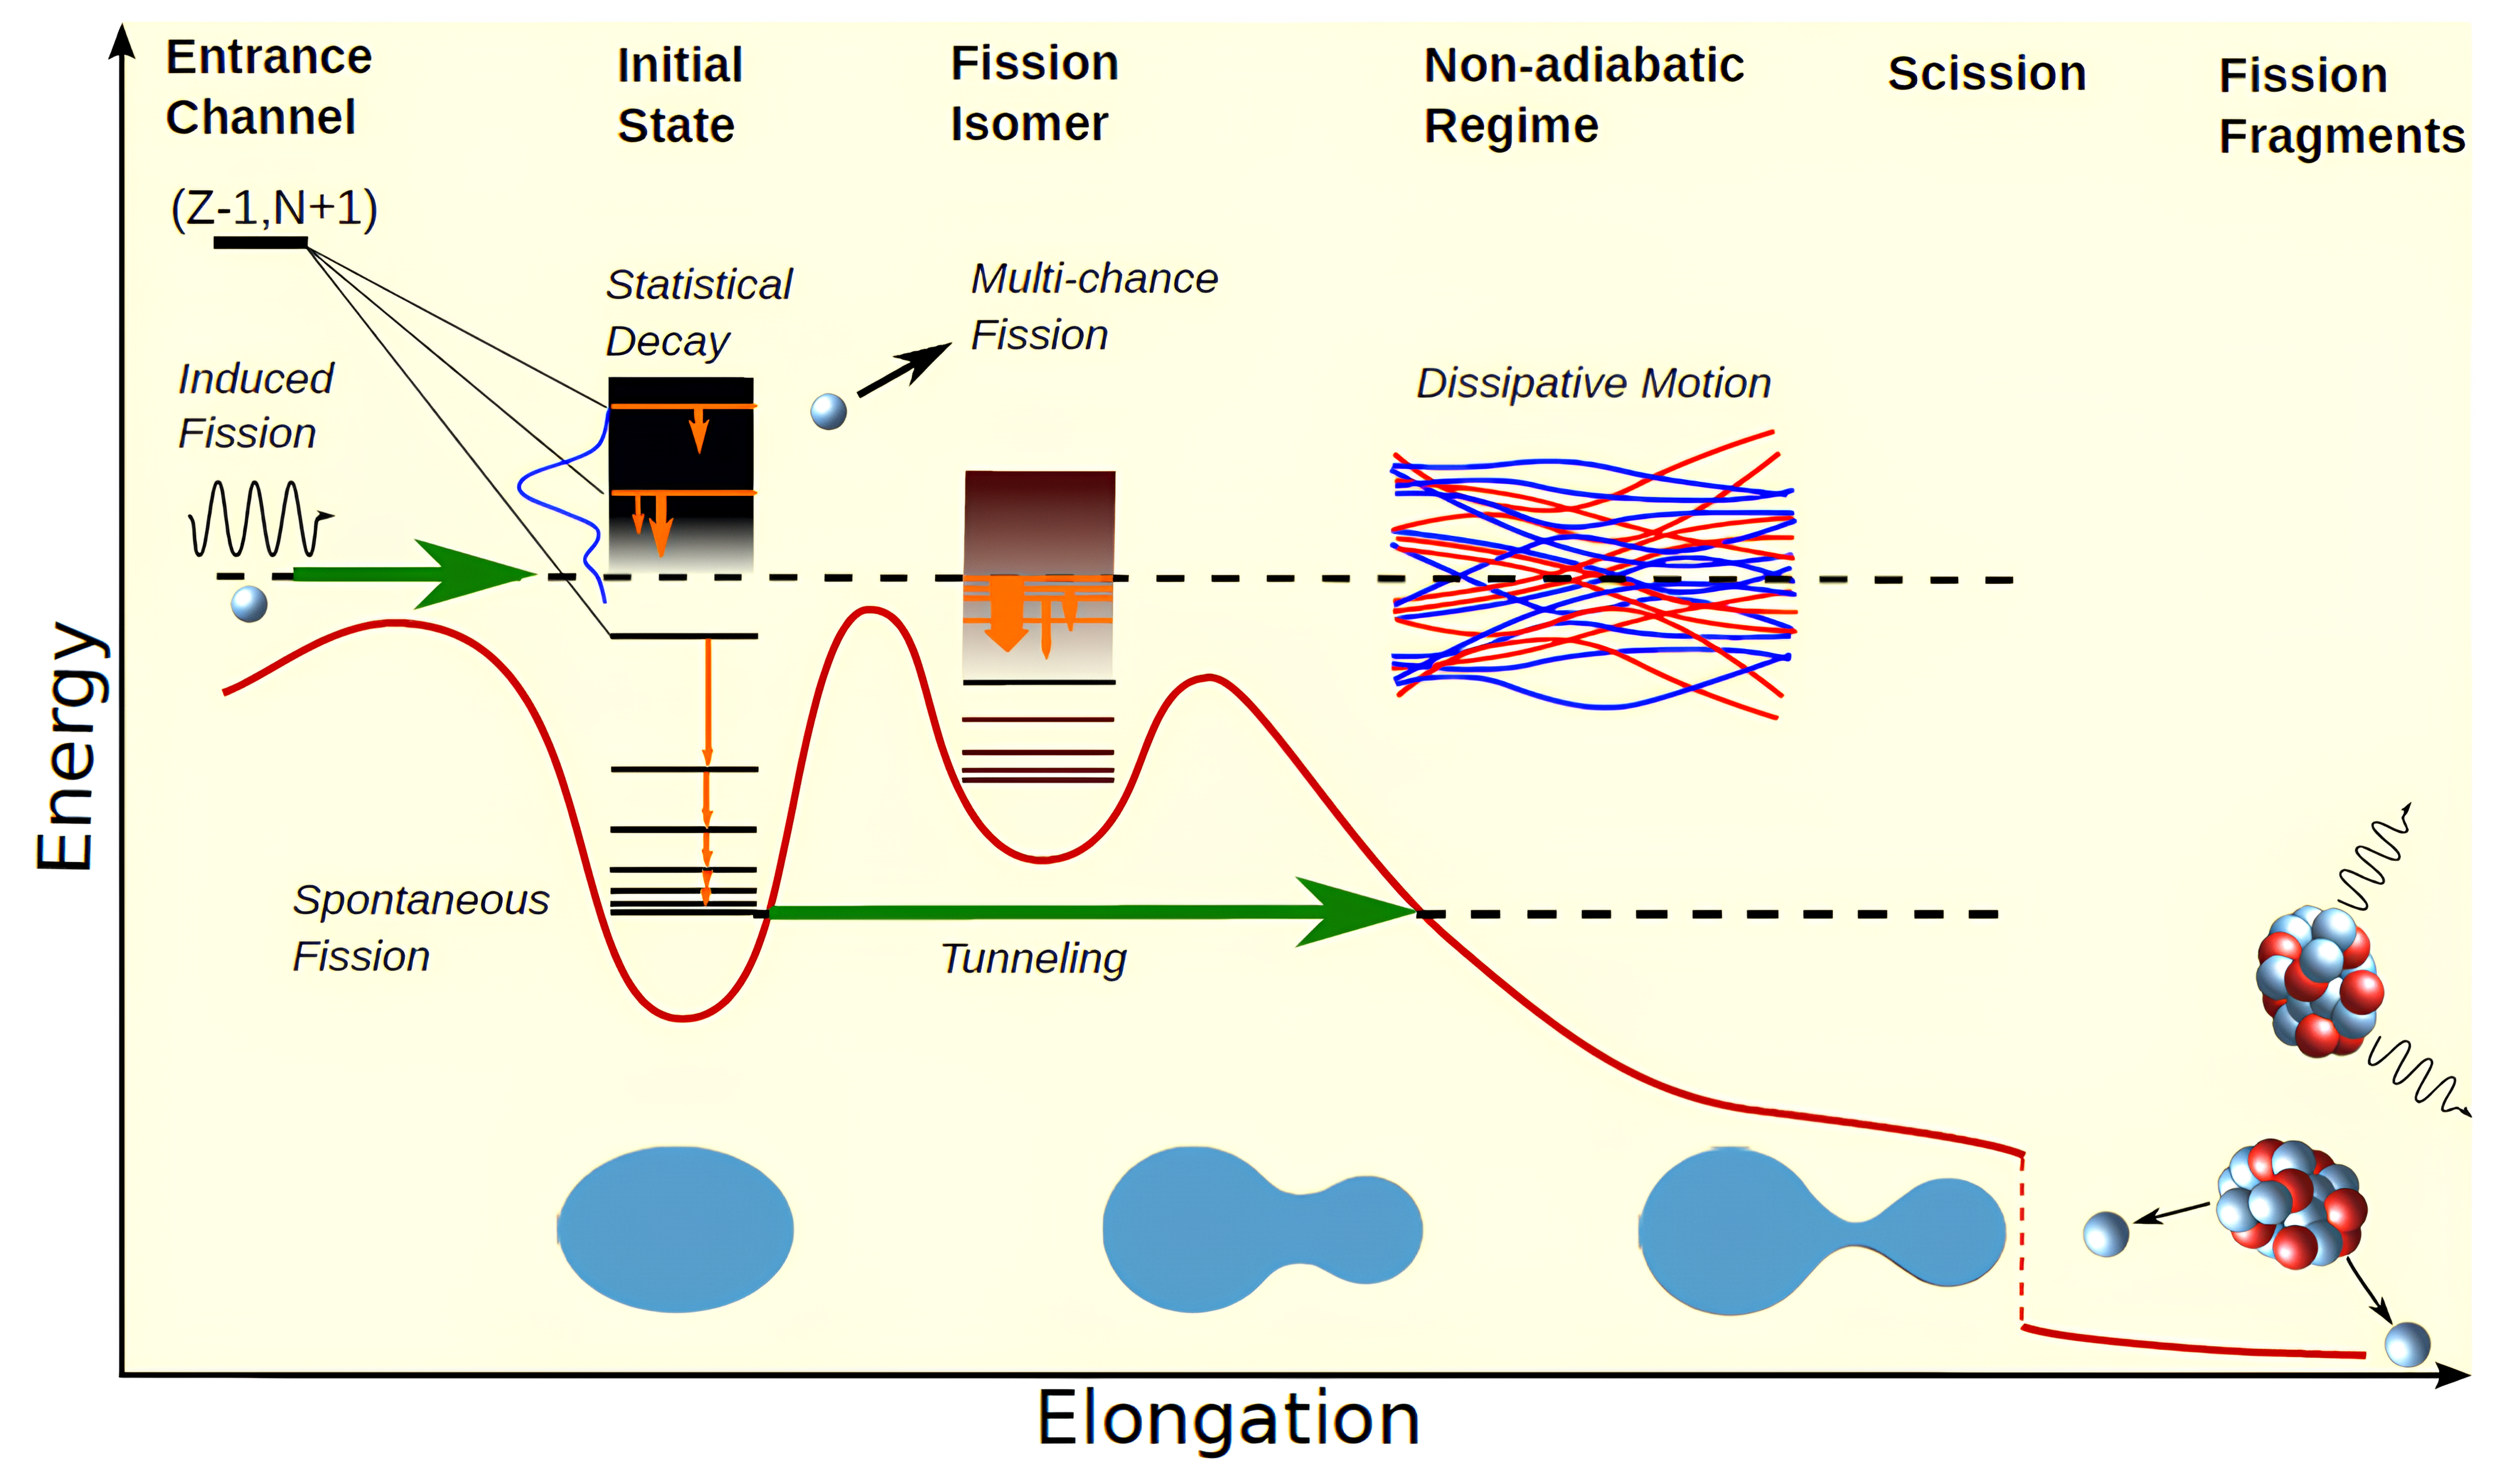
\includegraphics[width=0.85\textwidth]{Images/fission.png}
    \caption{Visual representation of the fission process. Figure taken from \cite{Bender2020}.}
    \label{fig:fission}
\end{figure}

\subsubsection{Spontaneous fission model}
It should be ovious that a formal treatment of deformations and collective modes is necessary to give a theoretical description of fission reactions. We can derive a simple spontaneous fission model by studying the effect of an axial quadrupole deformation on the semiempirical mass formula \ref{eq:semf}.

Let us assume that the nuclear radius may be expanded, as previously done in section \ref{sec:deformations}, as
\begin{equation}
    R = R_0[1+\alpha_{20}Y_{20}].
\end{equation}
Assuming the nuclear volume is conserved across the fission path, the volume energy will not change. As for the surface energy, its variation can be expressed at the lowest order in $\alpha_{20}$ as
\begin{equation}
    \Delta E_\text{surf} = E_\text{surf}
    -E_{0,\text{surf}} = E_{0, \text{surf}}\frac 2 5 \alpha_{20}^2.
\end{equation}
Regarding the Coulomb energy, the variation is given by
\begin{equation}
    \Delta E_\text{coul} = E_\text{coul} - E_{0, \text{coul}} = -E_{0, \text{coul}}\frac 1 5 \alpha_{20}.
\end{equation}
Since the neutron and proton numbers does not change, the surface and Coulomb energies are the only contributions to the total energy difference. We can write
\begin{equation}
    \label{eq:fission_semf}
    \Delta E = \frac 2 5 \alpha_{20}^2 a_s A^{2/3}- \frac 1 5 \alpha_{20}^2 a_c Z^2 A^{-1/3},
\end{equation}
if we set equation \eqref{eq:fission_semf} to zero, we get, other than the undeformed solution for $\alpha_{20}=0$, 
\begin{equation}
    \frac{ Z^2}{A} = \frac{2 a_s}{a_c},
\end{equation}
where the ratio $2a_s/a_c$ amounts to $\approx 50$ in typical parametrizations of the SEMF. Equation \eqref{eq:fission_semf}, shows that for values of the so called \textit{fissility parameter} $Z^2/A$ larger than $50$, the energy change becomes negative, favouring a configuration in which the nucleus fragments due to the spontaneous fission.
\subsection{Symmetry breaking and microscopic approaches to fission}
\subsubsection{Microscopic theory}
The use of phenomenological macroscopic-microscopic models has long provided valuable insight into fission processes, allowing for the prediction of barrier heights and fragment yields through parametrised shape degrees of freedom and empirical shell corrections \cite{Brack1972,Bjornholm1980,Krappe2012}.  
In these models, the total energy is expressed as
\begin{equation}
E_{\mathrm{tot}}(\boldsymbol{q}) = E_{\mathrm{LD}}(\boldsymbol{q}) + \delta E_{\mathrm{shell}}(\boldsymbol{q}) + \delta E_{\mathrm{pair}}(\boldsymbol{q}),
\end{equation}
where $E_{\mathrm{LD}}$ is the macroscopic liquid-drop term depending on deformation coordinates $\boldsymbol{q}$, while $\delta E_{\mathrm{shell}}$ and $\delta E_{\mathrm{pair}}$ account for shell and pairing corrections, respectively.  
While such models reproduce many global observables, they lack a true microscopic foundation.  
In particular, the collective coordinates $\boldsymbol{q}$ are not derived from the underlying many-body dynamics, and the empirical shell corrections cannot describe the self-consistent rearrangement of the mean field along the fission path.

A more fundamental understanding is achieved within self-consistent mean-field approaches such as the Hartree-Fock or Hartree-Fock-Bogoliubov formalisms. The use of nuclear Density Functional Theory \cite{Bender2003,Schunck2016} allows one to define a universal EDF $E[\rho,\kappa]$ that encapsulates both mean-field and pairing correlations.  
The resulting constrained HF/HFB calculations produce the potential energy surface (PES) $E(\boldsymbol{q})$, mapping the energy of the system as a function of collective deformations such as the quadrupole ($Q_{20}$), octupole ($Q_{30}$), and triaxial ($Q_{22}$) moments.  
The minima and saddle points of this multidimensional PES determine the fission barriers and shape isomeric states \cite{Dubray2012,Schunck2016}.

However, static mean-field approaches are limited by their single-reference character: the HFB vacuum represents only one configuration at a time, typically corresponding to a local minimum of the PES.  
In the vicinity of the fission barrier, where several configurations with different intrinsic quantum numbers coexist, this approximation breaks down.  
The wave function should instead be expressed as a superposition of several self-consistent configurations $\{|\Phi(\boldsymbol{q})\rangle\}$, leading to a correlated state of the form
\begin{equation}
|\Psi\rangle = \int f(\boldsymbol{q})\, |\Phi(\boldsymbol{q})\rangle\, d\boldsymbol{q},
\end{equation}
which is the essence of the \emph{Generator Coordinate Method} (GCM) \cite{Goutte2005,Regnier2019}.  
The GCM maps the microscopic many-body problem onto a \emph{collective Schrödinger equation} (CSE)
\begin{equation}
\left[ -\frac{\hbar^2}{2}\sum_{ij}\frac{\partial}{\partial q_i} B_{ij}(\boldsymbol{q}) \frac{\partial}{\partial q_j} + V(\boldsymbol{q}) \right] g_k(\boldsymbol{q})
= E_k g_k(\boldsymbol{q}),
\end{equation}
where $B_{ij}(\boldsymbol{q})$ is the collective inertia tensor and $V(\boldsymbol{q})$ the potential energy extracted from constrained HFB.  
This framework naturally incorporates tunnelling through the barrier and provides access to observables such as fission lifetimes and fragment distributions.  

Beyond-mean-field extensions also restore symmetries that are spontaneously broken at the mean-field level.  
For instance, particle-number, parity, and angular-momentum projection techniques \cite{Bender2004,Samyn2005} are required to recover good quantum numbers and remove spurious symmetry mixing.  
In multi-reference DFT \cite{Bender2003}, these symmetry restorations can be combined with configuration mixing, yielding highly accurate fission barrier calculations.  

\subsubsection{Unconstrained Calculations and Symmetry Breaking}

An equally important aspect of microscopic fission theory is the treatment of spatial symmetries.  
Historically, many calculations imposed constraints such as axial symmetry or reflection symmetry with respect to a plane to reduce the computational cost of solving the HFB equations.  
While such restrictions simplify the description of the nucleus, they artificially constrain the fission path and may even prevent the identification of energetically preferred configurations \cite{Warda2002,Bertsch2018}, as shown in figure \ref{fig:fission_barrier}.  
Fission involves strongly deformed, triaxial, and reflection-asymmetric shapes; the correct description of barrier heights and scission configurations therefore requires breaking as many spatial symmetries as possible.

In the self-consistent mean-field framework, spontaneous symmetry breaking is a feature rather than a flaw: it allows the system to adopt a deformed intrinsic shape corresponding to a broken rotational or parity symmetry, while the symmetry of the total many-body Hamiltonian is preserved.  
For example, an axially deformed HFB state violates rotational invariance, but the restoration of this symmetry through angular-momentum projection recovers the correct laboratory-frame properties.  
Similarly, parity breaking through octupole deformation is essential to describe asymmetric fission fragment distributions. Triaxiality, for example, has been shown to lower the inner barrier of actinides by several MeV \cite{Warda2002,Schunck2016}.
Likewise, reflection-asymmetric (octupole) degrees of freedom are necessary to reproduce mass-asymmetric fission in heavy nuclei.

Recent computational developments have made possible fully symmetry-unrestricted HFB and TDDFT calculations, in which all spatial and time-reversal symmetries can be broken if energetically favourable \cite{Simenel2018,Schunck2016}.  
Codes such as \texttt{HFODD} and \texttt{Sky3D} implement three-dimensional solvers capable of describing triaxial, octupole, and time-odd components of the density matrix.  
These advances have revealed new fission pathways, scission configurations, and fragment-spin correlations inaccessible to axially symmetric models.

In summary, microscopic theories based on DFT and its extensions offer a self-consistent foundation for the description of nuclear fission.  
They provide direct access to the interplay between shell effects, pairing, and deformation, which determine the shape evolution from the ground state to scission.  
